\documentclass[11pt]{article}
\usepackage[utf8]{inputenc}
\usepackage{amsmath}
\usepackage{amsfonts}
\usepackage{amssymb}
\usepackage{graphicx}
\usepackage{float}
\usepackage{hyperref}

\usepackage{todonotes}

\usepackage{rsfso} %Add the fancy L used in lagrange
\usepackage{siunitx}

\newcommand{\thomas}[1]{\todo[inline,color=black!30]{Thomas: #1}}
\newcommand{\mikkel}[1]{\todo[inline,linecolor=green!100,backgroundcolor=red!70, bordercolor=green]{Mikkel: #1}}

%Information to be included in the title page:
\title{Real-Time Systems}
\author{Thomas S. Christensen, Mikkel Skaarup Jaedicke}
\date{Jan, 2017}

\begin{document}
\input{sections/test_bed.tex}
\newpage
%!TEX root = ../main.tex

\section{Model Development} % (fold)
\label{sec:model_development}

In order to properly control the double pendulum it is necessary to develop a model of the system.
Throughout this section the model will be developed iteratively.
Initially including only the simple double pendulum, eventually including both friction and the cart.

\subsection{Simple Double Pendulum} % (fold)
\label{sub:simple_double_pendulum}
An illustration of the system can be seen in figure \ref{fig:doublependulum}.
As can be seen, the pendulums have masses $m_1$, $m_2$, suspended using rods of lengths $l_1$, $l_2$.
The rods are assumed to be massless.
The angles of the pendulums $\theta_1$, $\theta_2$, are measured as the offset from the stable position.
For convenience the two pendulums will be referred to as $p_1$ and $p_2$ where $p_2$ is suspended from $p_1$.

\begin{figure}
	\centering
	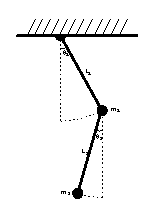
\includegraphics[width=.5\linewidth]{graphics/double_pendulum.eps}
	\caption{Illustration of the simple double pendulum.}
	\label{fig:doublependulum}
\end{figure}

\mikkel{Maybe the illustration needs to be changed in order properly show the positive direction of $\theta_2$ }

Equations should be developed such that, given an initial state, the position and subsequent movement can be derived from them.
This can be achieved using the Euler-Lagrange differential equations.
These will be found for this system throughout the remainder of this section.
Firstly, the position of the pendulums as a function of the angle must be determined.
The pendulums are placed in the x-y plane with the origin placed at the point of suspension of $p_1$.
When the pendulums are in the stable position, $\theta_1=\theta_2=0$, they are aligned with the y-axis.
The x-axis is positive to the right of the stable position.
The coordinates of $p_1=(x_1,y_1)$ and $p_2=(x_2,y_2)$ are as follows:
\begin{align}
	x_1 &= l_1\sin{\theta_1}\\
	y_1 &= -l_1\cos{\theta_1}\\
	x_2 &= l_1\sin{\theta_1} + l_2\sin{\theta_2}\\
	y_2 &= -l_1\cos{\theta_1} - l_2\cos{\theta_2}
\end{align}
While the derivatives are not used until later, they are presented here for clarity:
\begin{align}
	\dot{x}_1 &= l_1\cos{\theta}_1\dot{\theta}_1\\
	\dot{y}_1 &= l_1\sin{\theta}_1\dot{\theta}_1\\
	\dot{x}_2 &= l_1\cos{\theta}_1\dot{\theta}_1 + l_2\cos{\theta_2}\dot{\theta}_2\\
	\dot{y}_2 &= l_1\sin{\theta}_1\dot{\theta}_1 + l_2\sin{\theta_2}\dot{\theta}_2
\end{align}
In order to calculate the Euler-Lagrange diff. eq. it is necessary to first determine the lagrangian, $\mathcal{l}$:
\begin{equation}
	\mathcal{L}=E_k-E_p
\end{equation}
Where $E_k$ is the kinetic energy of the system and $E_p$, the potential energy.
The derivation of $E_p$:
\mikkel{g being the standard acceleration due to gravity}
\begin{align}
	E_p &= m_1 g y_1 + m_2 g y_2\\
		&= -m_1 g l_1 \cos{\theta_1} - m_2 g l_1 \cos{\theta_1} - m_2 g l_2 \cos{\theta_2}\\
		&= -(m_1+m_2)l_1g \cos{\theta_1}-m_2 g l_2 \cos{\theta_2}
		\label{eq:ep}
\end{align}
The derivation of $E_k$:
\begin{equation}
	\label{eq:ek}
	E_k = \frac{1}{2}m_1v_1^2+\frac{1}{2}m_2v_2^2
\end{equation}
As movement is present along both axes, the total velocity of either pendulum can be found as the derivative of the position and Pythagoras:
\begin{align}
	v_1^2 &= \dot{x}_1^2+\dot{y}_1^2\\
		&= l_1^2\dot{\theta}_1^2\cos{\theta}_1^2+l_1^2\dot{\theta}_1^2\sin{\theta_1}^2\\
		&= (\cos{\theta_1}^2+\sin{\theta_1}^2)l_1^2\dot{\theta}_1
\end{align}
Using the Pythagorean identity:
\begin{equation}
	\label{eq:v1}
	v_1^2 = l_1^2\dot{\theta}_1^2
\end{equation}
Similarly:
\begin{align}
	v_2^2 &= \dot{x}_2^2+\dot{y}_2^2\\
	&= (l_1\cos{\theta}_1\dot{\theta}_1 + l_2\cos{\theta_2}\dot{\theta}_2)^2+(l_1\sin{\theta}_1\dot{\theta}_1 + l_2\sin{\theta_2}\dot{\theta}_2)^2\\
	\begin{split}
		&= l_1^2\dot\theta_1^2\cos{\theta_1}^2+l_2^2\dot\theta_2^2\cos{\theta_2}^2+2l_1l_2\dot\theta_1\dot\theta_2\cos{\theta_1}\cos{\theta_2}\\
		&\qquad +l_1^2\dot\theta_1^2\sin{\theta_1}^2+l_2^2\dot\theta_2\sin{\theta_2}+2l_1l_2\dot\theta_1\dot\theta_2\sin{\theta_1}\sin{\theta_2}
	\end{split}
\end{align}
Isolating cosine and sine from the terms pairwise, 1 and 4, 2 and 5, 3 and 6, yields:
\mikkel{from equation 20? add in text}
\begin{align}
	\begin{split}
		v_2^2&=(\cos{\theta_1}^2+\sin{\theta_1}^2)l_1^2\dot\theta_1^2+(\cos{\theta_2}^2+\sin{\theta_2}^2)l_2^2\dot\theta_2^2\\
	&\qquad+(\cos{\theta_1}\cos{\theta_2}+\sin{\theta_1}\sin{\theta_2})2l_1l_2\dot\theta_1\dot\theta_2
	\end{split}
\end{align}
By applying the trigonimetric identities:
\begin{align}
	1&=\sin{\alpha^2}+\cos{\beta^2}\\
	\cos{(\alpha\pm\beta)}&=\cos\alpha\cos\beta\mp\sin\alpha\sin\beta
\end{align}
The result is found:
\begin{equation}
	\label{eq:v2}
	v_2^2=l_1^2\dot\theta_1^2+l_2^2\dot\theta_2^2+2l_1l_2\dot\theta_1^2\dot\theta_2^2\cos{(\theta_1-\theta_2)}
\end{equation}
Using equations \ref{eq:ep}, \ref{eq:ek}, \ref{eq:v1} and \ref{eq:v2} the lagrangian can be constructed:
\begin{align}
	\begin{split}
		\mathcal{L}&=\frac{1}{2}m_1l_1^2\dot\theta_1^2+\frac{1}{2}m_2\left(l_1^2\dot\theta_1^2+l_2^2\dot\theta_2^2+2l_1l_2\dot\theta_1^2\dot\theta_2^2\cos{(\theta_1-\theta_2)}\right)\\
		&\qquad+(m_1+m_2)l_1g\cos{\theta_1}+m_2l_2g\cos{\theta_2}
	\end{split}\\
	\begin{split}
		&=\frac{m_1l_1^2\dot\theta_1^2}{2}+\frac{m_2l_1^2\dot\theta_1^2}{2}+\frac{m_2l_2^2\dot\theta_2^2}{2}+l_1l_2\dot\theta_1\dot\theta_2\cos{(\theta_1-\theta_2)}\\
		&\qquad+(m_1+m_2)l_1g\cos{\theta_1}+m_2l_2g\cos{\theta_2}
	\end{split}
\end{align}
Which simplifies to:
\begin{equation}
	\label{eq:lagrangian}
	\begin{split}
		\mathcal{L}=\frac{(m_1+m_2)l_1^2\dot\theta_1^2}{2}+\frac{m_2l_2^2\dot\theta_2}{2}+l_1l_2\dot\theta_1\dot\theta_2\cos{(\theta_1-\theta_2)}\\
		+(m_1+m_2)l_1g\cos{\theta_1}+m_2l_2g\cos{\theta_2}\\
	\end{split}
\end{equation}
The Euler-Lagrange diff. eq. are defined as:
\begin{equation}
	\frac{d}{dt}\left(\frac{\partial \mathcal{L}}{\partial \dot\theta}\right)-\frac{\partial \mathcal{L}}{\partial \theta} = 0
\end{equation}
The three terms $\frac{\partial \mathcal{L}}{\partial \dot\theta}$,$\frac{d}{dt}\left(\frac{\partial \mathcal{L}}{\partial \dot\theta}\right)$ and $\frac{\partial l}{\partial \theta}$ are calculated next for each of the pendulums. 
\\For $p_1$:
\begin{align}
	\frac{\partial \mathcal{L}}{\partial \dot\theta_1}&=(m_1+m_2)l_1^2\dot\theta_1+m_2l_1l_2\dot\theta_2\cos{(\theta_1-\theta_2)}\\
	\begin{split}
		\frac{d}{dt}\left(\frac{\partial \mathcal{L}}{\partial \dot\theta_1}\right)&=(m_1+m_2)l_1^2\ddot\theta_1+m_2l_1l_2\ddot\theta_2\cos{(\theta_1-\theta_2)}\\
		&\qquad-m_2l_1l_2\dot\theta_2\sin{(\theta_1-\theta_2)(\dot\theta_1-\dot\theta_2)}
	\end{split}\\
	\frac{\partial \mathcal{L}}{\partial \theta_1} &= -m_2l_1l_2\dot\theta_1\dot\theta_2\sin(\theta_1-\theta_2)-(m_1+m_2)l_1g\sin{\theta_1}\\
\end{align}
\mikkel{Entering the x,x,x equations yields the first the Euler-Lagrange diff bla bla.}
\begin{align}
	\begin{split}
		0&=(m_1+m_2)l_1\ddot\theta_1+m_2l_2\ddot\theta_2\cos{(\theta_1-\theta_2)}\\
		&\qquad+m_2l_2\dot\theta_2^2\sin{(\theta_1-\theta_2)}+(m_1+m_2)g\sin{\theta_1}
	\end{split}
\end{align}
And $p_2$:

\begin{align}
	\frac{\partial \mathcal{L}}{\partial \dot\theta_2}&=m_2l_2^2\dot\theta_2+m_2l_1l_2\dot\theta_1\cos{(\theta_1-\theta_2)}\\
	\begin{split}
		\frac{d}{dt}\left(\frac{\partial \mathcal{L}}{\partial \dot\theta_2}\right)&=m_2l_2^2\ddot\theta_2+m_2l_1l_2\ddot\theta_1\cos{(\theta_1-\theta_2)}\\
		&\qquad -m_2l_1l_2\dot\theta_1\sin{(\theta_1-\theta_2)}(\dot\theta_1-\dot\theta_2)
	\end{split}\\
	\frac{\partial \mathcal{L}}{\partial \theta_2} &=m_2l_1l_2\dot\theta_1\dot\theta_2\sin{(\theta_1-\theta_2)}-m_2l_2g\sin{\theta_2}\\
	\label{eq:part}
\end{align}
\mikkel{Entering the x,x,x equations yields the second the Euler-Lagrange diff bla bla.}
\begin{align}
	\begin{split}
		0&=m_2l_2\ddot\theta_2+m_2l_1\ddot\theta_1\cos{(\theta_1-\theta_2)}\\
		&\qquad-m_2l_1\dot\theta_1^2\sin{(\theta_1-\theta_2)}+m_2g\sin{\theta_2}
	\end{split}
\end{align}
\thomas{eq. \ref{eq:part} has a minus in front of the first term according to our calculations. Determine why.}
% subsection simple_double_pendulum (end)

% section model_development (end)

\newpage
%!TEX root = ../main.tex
\section{The Platform} % (fold)
\label{sec:the_platform}
A new platform was made available to the project which fulfilled many of the requirements set by the application.
It consists of a cart, driven by a timing belt, mounted on an aluminium rail.
An image of the platform can be seen in figure \ref{fig:platform}.
\mikkel{Maybe mention what it was used for before?}
\begin{figure}[H]
 	\centering
 	\missingfigure{Image of the platform}
 	%\includegraphics[width=\linewidth]{graphics/platform}
 	\caption{The platform used in the project.}
 	\label{fig:platform}
 \end{figure} 
% section the_platform (end)
%!TEX root = ../main.tex
\section{Preliminary Testing} % (fold)
\label{sec:preliminary_testing}
In an effort to split the development into smaller, more managable parts, it was decided to initially develop the system such that it fulfills the following requirements:

\begin{itemize}
	\item The cart should be able to move with known position.
	\item Endstops on the platform should stop movement.
	\item Emergency button should stop movent.
\end{itemize}

Clearly, making the cart move is crucial in the development of the system and forms the basis for any later developments.
The latter two requirements are related to the safe operation of the platform.
It is expected that at least during development, an error may occur that causes the cart to move uncontrollably.
In such a situation the programmer should be able to completely shut off power to the motor.
The endstops will ensure that a minimum of mechanical or electrical damage is incurred on the platform in case of a cart crash.
The following paragraphs will explore what is required in order to fulfill the above requirements.
\subsection{Safety Circuitry} % (fold)
\label{sub:safety_circuitry}
Safety first.
A safety system should, whenever possible, be isolated from the remaining system.
That is, it should depend on non of the remaining circuitry or programming.
Usually, if it can at all be avoided, no programming should be involved in determining a safety condition.
With this in mind, the safety system for this platform should be designed in such a way that, when activated, it will cut power to the motors.
In order to more easily identify the cause of the fault, the remaining electronics should remain operational to maintain the current program status.
\\~\\
Creating the endstops can be done in a multitude of ways.
In this project three approaches were considered:
\paragraph{Mechanical Switch:} % (fold)
\label{par:mechanical_switch}
The simplest form of switch is the mechanical switch.
The switch should be mounted in such a way that the cart would move into the switch, therefore activating it.
This approach is not without issues.
Firstly, the simplest mounting solution would require the switch to be mounted in the direct path of the cart.
If the cart is traveling at full speed it is unlikely that the cart would stop before crashing into the switching mechanism, potentially damaging it.
A switch mounted in this fashion would need to be rather robust.
Some other mounting solutions could be thought of that do not suffer from this problem, especially if a flexible microswitch is used.
These types of switches can be fragile and may not be sufficiently durable, considering the usecase.
All mechanical switches have one drawback in common: they are mechanical.
Generally, mechanical items wear out over time and require maintainance or replacement.
% paragraph mechanical_switch (end)
\paragraph{Hall Effect Sensor:} % (fold)
\label{par:hall_effect_sensor}
This type of sensor measures magnetic fields and produces a voltage proportional to the strength of the field.
By placing a small neodymium magnet on the cart and mounting a hall effect sensor on the rail in such a way that the coincide would allow for detecting when the cart is above the sensor.
If the sensor is combined with a schmitt-trigger circuit the output could be a binary result, either the endstop is reached or it is not.
Using this method requires that a magnet is placed on the cart itself and that a sensor is mounted to the rail.
It should be noted that accelerating rather strong magnetic fields back and forth on the platform may not be the least electrically noisy solution one could think of.
Magnetic fields are also wide, meaning that the cart would "sneak up on" the threshold.
This requires some amount of calibration to determine the correct distance between sensor and magnet, which may not be mechanically simple to determine. 
% paragraph hall_effect_sensor (end)
\paragraph{Infrared Transceiver:} % (fold)
\label{par:infrared_transceiver}
This type of device is a combined LED and infrared sensor.
The LED is optimised for emitting infrared light, or radiation (IR), and the sensor for sensing it.
The LED emits IR outward from the device which, when an object is placed in front of it, will bounce off the object and be caught by the sensor.
As with the hall effect sensor, this type of device produces a voltage output proportional to the amount of IR being sensed and as such a schmitt-trigger circuit would also be benficial in this case.
With this sensor type it is important to realise that the LED will not be the only emitter of IR in the vicinity.
Any type of lamp will emit IR, especially glowbulbs (of which there are few left, luckily) but also sunlight contains some amount of IR.
When using this sensor the circuit should be designed in such a way that only the effect of the IR radiated back on the sensor will trigger the circuit.
The sensor should be mounted immediately below the cart so as to maximize the radiated IR and therefore the signal strength.
% paragraph infrared_transceiver (end)
\\~\\
While all of the above have their drawbacks, it was decided to use the infrared transceiver.
This sensor allows the greatest reliability while being reasonably simple to mount on the platform in that it requires no modification to the cart.
\\~\\
In addition to the endstops, also an emergency button, preferably red, should be able to cut power to the motors.
It may be that additional safety features are added later.
In order to minimize the amount of circuitry, all safety features will trip the same circuit.
\thomas{Add circuit showing the safety relay}
On figure \ref{fig:relay_circuit} is shown the safety circuitry.
A relay is mounted in series with the supply rail for the motor.
The default state for this relay should be \texttt{off}.
Then, in order to switch the system to the \texttt{on} state, the relay should be closed.
Should power to the relay coil ever fail i.e. something in the system has broken, power to the motor is cut off.
Since the relay is in series with the motor, it should also be capable of carrying the full design current, 80A.
One relay that fulfills these requirements is the.
\\~\\
The driver circuit for the relay is activated only when all safety conditions are off.
If at any point any of the safety conditions are tripped, the driver circuit shuts down, releasing the relay and turning off power to the motor.
Designing the safety circuit in this manner ensures that the system cannot be started or will shut down if any wires or components in the safety circuit break.

% subsection safety_circuitry (end)
\subsection{Power Board} % (fold)
\label{sub:power_board}
it is necessary to device some form of driving circuitry for the motor driving the timing belt.
On the platform is a Maxon 148867 Brushed DC Motor.
This is a 150W motor with a nominal current of 6A and a stall current of 80A.
Clearly, the system should under normal use not come anywhere close to stalling the motor but considering the use case, experimentation with control from students, it may be beneficial to design the circuitry such that it can withstand being stalled, for at least a short period of time.
In order to reach this goal, it is necessary to size the components for at least some amount above 80A continuous.
The \texttt{IPP045N10N3} MOSFET \cite{mosfet} is a 100V/100A MOSFET.
It is made in the standard TO-220 housing.
This housing allows for easy mounting of a heatsink and due to its wide application, there are many shapes and sizes to choose from.
Table \ref{tab:mosfetparameters} holds a list of the relevant parameters.

\begin{table}[tb]
	\centering
	\begin{tabular}{|r|c|c|c|}
	\hline
		\textbf{Parameter} & \textbf{Min} & \textbf{Typ} & \textbf{Max} \\
	\hline
		$V_{\text{th}}$ [V] & 2 & 2.7 & 3.5 \\
	\hline
		$R_{\text{ds(on)}}$ [m$\Omega$]& - & 3.6 & 4.2 \\
	\hline
		$Q_\text{g}$ [nC] & - & 88 & 117 \\
	\hline
		$I_\text{d}$ [A] & - & 100 & - \\
	\hline
		$V_{\text{ds}}$ [V] & 100 & - & - \\
	\hline
	\end{tabular}
	\caption{Relevant parameters of the IPP045N10N3 MOSFET \cite{mosfet} chosen for the full-bridge.
	Here, \vth is the gate threshold voltage, \ron is the drain-source on resistance, \qg is the total gate charge, \id is the maximum continuous drain current and \vds is the minimum guaranteed drain-source breakdown voltage.}
	\label{tab:mosfetparameters}
\end{table}

It should be noted that even though \vth is maximum 3.5V, this is not enough to fully open the MOSFET.
Rather, this voltage is where the MOSFET will start to conduct.
Figure \ref{fig:mosfettransfercharacteristic} reveals that the MOSFET is not fully conducting until \vgs $>4.5$V.

\begin{figure}[H]
	\centering
	\includegraphics[width=.5\linewidth]{graphics/mosfet_transfer_characteristic}
	\caption{Transfer characteristic of the IPP045N10N3 as per the datasheet.
	Inspecting the graph reveals that the maximum \id of 100A is reached at \vgs$\approx4.5\rightarrow4.75$V.}
	\label{fig:mosfettransfercharacteristic}
\end{figure}

The motor should be able to move in both directions so an h-bridge, or full-bridge is required.
By properly switching the MOSFETs in the circuit on and off the average voltage across the motor can be controlled and therefore also the speed and direction of the motor, see \ref{sec:hbridge} for more details.
\\~\\
\thomas{Insert reference to note on full-bridge drive}
Having chosen a MOSFET for the full-bridge, some form of driver must be designed for the full-bridge.
For this task, ready-made full-bridge drivers exist on the market that incorporate all of the electronics required to generate the driving signals, requiring only a PWM signal from the designer.
In order to choose one, a few parameters must be fulfilled.

\begin{itemize}
	\item \textbf{Output Current:} The amount of current necessary to properly drive the MOSFET.
	This value depends on the switching frequency of the application, the gate-to-source voltage ($V_{gs}$) and the total gate charge of the MOSFET.
	\item \textbf{Driving Voltage:} In order to ensure that the MOSFET is turned on quickly and fully the driver should be able to supply a voltage well above the gate threshold of the MOSFET.
	\item \textbf{High-Side Drive Capabilities:} The high side MOSFET of the full-bridge is referenced not to ground, but to $V_{\text{cc}}$.
	This means that in order to switch on this MOSFET $V_{\text{gs}}$ must be at least $V_{\text{cc}}+V_{\text{th}}$ where $V_{\text{th}}$ is the gate threshold voltage of the MOSFET.
	This is bootstrapping and is explained in more detail in section \ref{sec:bootstrap}.
	\item \textbf{Shoot-Through Protection and Deadtime:} Due to the structure of the full-bridge it is important that two MOSFETs on the same half-bridge are never on at the same time as this would result in a short from $V_{\text{cc}}$ to ground.
	This is resolved with a combination of deadtime (a delay where no MOSFET is on) and a logic table that ensures that an illegal switch combination can never happen.
\end{itemize}

The HIP4081AIBZ \cite{driver} full-bridge driver meets all of the above requirements.
It can supply up to 2.5A on the output pins with a voltage approximately 1V below \vcc, well above the required \vth.
Since the motor should, preferably, be driven outside the audible frequency range, it was chosen to set the switching frequency at 22kHz.
This frequency was chosen over an even higher frequency because increasing the frequency also increases the switching losses.
At this frequency there is $\frac{1}{22000}\approx45\mu$S per cycle. 
Well within this time the gate should be fully opened.
Since:

\begin{equation}
	I = C\frac{\text{dv}}{\text{dt}} \quad\Rightarrow\quad \text{dt} = C\frac{\text{dv}}{I}
\end{equation}
\thomas{Is this the correct way of calculating it?}

Accounting for various voltage drops it is assumed that \vgs is 10V, a rough estimate of the time to open the gate completely can be found as:

\begin{equation}
	\text{dt} = 117\cdot10^{-9}\frac{10}{2.5}\approx0.47\mu\text{S}
\end{equation}

This time is approximately 100 times shorter than the allotted time frame.
The component also has floating drive circuitry, meaning that by referencing the high-side driver to source of the high-side MOSFET, the driver can be made to output a voltage higher than \vcc.
This does require a few external components for the bootstrapping.
The choice of these components and a more in depth explanation of the procedure is given in section \ref{ssub:bootstrap_circuit}.
Finally, the component has a user-programmable dead time and shoot-through protection. 

HIP4081AIBZ - Full-bridge driver - (ISL83202)

IPP045N10N3 - Mosfet

choice of VGS, 8V - show graph of transfer characteristics of mosfet, high due to uncertainty.
% subsection power_board (end)
% section preliminary_testing (end)

%!TEX root = main.tex
\begin{thebibliography}{21} %This number should be higher than the number of entries in the bibliography because reasons...
%	\bibitem{id}
%		Author(s) Last name, First name, Company/Organisation, Year. Full Title
\bibitem{hedg9000}
	Avago Technologies, August 2011, HEDG-9000 Series - Codewheel for use with Avago Technologies - Ultra-precision 17-Bit Absolute Single Turn Encoder
Encoder Modules AEAT-9000 series
\bibitem{aeat9000}
	Avago Technologies, April 2012, AEAT-9000-1GSH1 (Basic Option) - Ultra-precision 17-Bit Absolute Single Turn Encoder
\bibitem{mosfet}
	Infineon, August 2016, IPP045N10N3 Datasheet Rev. 2.8, \url{http://www.infineon.com/dgdl/Infineon-IPP045N10N3G-DS-v02_08-EN.pdf?fileId=db3a30431ce5fb52011d1e8b0cc31586}
\bibitem{bootstrap_ON}
	ON Semiconductor, December 2014, Design and Application Guide of Bootstrap Circuit forHigh-Voltage Gate-Drive IC, \url{https://www.fairchildsemi.com/application-notes/AN/AN-6076.pdf}
\bibitem{bootstrap_infineon}
	A. Merello, A. Rugginenti, M. Grasso, International Rectifier, Using Monolithic High Voltage Gate Drivers, \url{http://www.infineon.com/dgdl/Infineon-Using+Monolithci+Voltage+Gate+Drivers-UM-v01_00-EN.pdf?fileId=5546d462584d1d4a01585242c11947b1}
\bibitem{diode_ds}
	Surface Mount Ultrafast Rectifier, April 2014, \url{http://docs-europe.electrocomponents.com/webdocs/1405/0900766b81405c8a.pdf}
\end{thebibliography}
\end{document}